\documentclass{standalone}
%\usepackage{import}
%\subimport{.../}{preamble}
\usepackage{tikz, graphicx, cmbright}
\begin{document}
\fontsize{10pt}{1em}\selectfont

\begin{tikzpicture}
\node [above right] at (0, 0) {\includegraphics{tip_dimer_diagram.png}};
\node at (3.95, 0.3) {$d$};
\draw (3.8, 0.4) -- (3.8, 2.1);
\draw (4.1, 0.4) -- (4.1, 2.1);
\draw[->] (3.4, 0.45) -- (3.8, 0.45);
\draw[->] (4.5, 0.45) -- (4.1, 0.45);
\node at (3.4, 1.5) {$R$};
\draw[->]  (3.05, 1.3) -- (3.5,1.9);
\node at (3, 2.4) {$dz$};
\draw[->] (2.7, 2.2) -- (3.3, 2.2);
{\fontsize{7pt}{1em}\selectfont
\node at (2.6, 0.9) {$-$};
\node at (2.6, 1.7) {$-$};
\node at (3.65, 1.3) {$+$};
\node at (4.3, 1.3) {$-$};
\node at (5.3, 0.9) {$+$};
\node at (5.3, 1.7) {$+$};
}
\node[rotate=30] at (6, 2.8) {$\vec{k}_{in}$};
\draw[->] (7, 3) -- (5, 2.2);
\draw[->] (4.8, 2.2) -- (5.7, 3);
\node[rotate=45] at (5.15, 2.8) {$\vec{k}_{scat}$};
\end{tikzpicture}

\end{document}